\chapter{Massa en volume}\label{ch:g6:mass-and-volume}

Hoeveel limonade past er in de fles, en hoe zwaar is de krat met
flessen? Twee verschillende vragen --- ruimte en stof --- die de
alledaagse taal opgewekt tot één woord verstrengelt: ``groot''. De
wetenschap ontwart ze: \omterm{def:g6:mass-and-volume:volume}{volume} voor de ruimte die iets inneemt,
\omterm{def:g3:measuring-mass:mass}{massa} voor de stof die het bevat. In het \omterm{def:g6:measurement-in-science:measuring}{meten} van het tweede ben je
een oude rot; vandaag leren we het eerste te \omterm{def:g6:measurement-in-science:measuring}{meten} --- zelfs voor een
kiezelsteen zonder vorm waar een liniaal van kan houden.

\section{Volume: de ruimte die iets inneemt}

\begin{definition}[Volume]\label{def:g6:mass-and-volume:volume}
Het \emph{volume}\index{volume} van iets is de hoeveelheid ruimte die
het inneemt. Vaste stoffen, vloeistoffen en gassen hebben allemaal
volume: de baksteen neemt zijn ruimte, de limonade neemt de binnenkant
van de fles, de \omterm{def:g2:air-around-us:air}{lucht} neemt de rest. Volume wordt gemeten in
\emph{kubieke centimeters}\index{kubieke centimeter} (\unit{cm^3}) ---
de ruimte van een kubusje van één \omterm{def:g2:measuring-length:units}{centimeter} langs elke ribbe --- en in
\emph{liters}\index{liter} (\unit{L}).
\end{definition}

\begin{proposition}[De liter in kubusjes]\label{prop:g6:mass-and-volume:litre}
De twee families volume-eenheden zijn één familie:
\[
\qty{1}{L} = \qty{1000}{cm^3},
\qquad
\qty{1}{mL} = \qty{1}{cm^3}.
\]
Een \omterm{def:g6:mass-and-volume:volume}{liter} is precies de ruimte in een kubus van tien
\omterm{def:g2:measuring-length:units}{centimeter} langs elke ribbe: $10 \times 10 \times 10 = 1000$
kubusjes.
\end{proposition}

\begin{omfigure}
\begin{tikzpicture}[scale=0.85]
  \draw[thick] (0,0) rectangle (3,3);
  \draw[thick] (0,3) -- (0.9,3.75) -- (3.9,3.75) -- (3,3);
  \draw[thick] (3.9,3.75) -- (3.9,0.75) -- (3,0);
  \foreach \i in {1,...,9} {
    \draw[very thin] (0,0.3*\i) -- (3,0.3*\i);
    \draw[very thin] (0.3*\i,0) -- (0.3*\i,3);
    \draw[very thin] (0.3*\i,3) -- (0.3*\i+0.9,3.75);
    \draw[very thin] (3,0.3*\i) -- (3.9,0.3*\i+0.75);
    \draw[very thin] (0.09*\i,3+0.075*\i) -- (3+0.09*\i,3+0.075*\i);
    \draw[very thin] (3+0.09*\i,0.075*\i) -- (3+0.09*\i,3+0.075*\i);
  }
  \draw[thick, fill=omDef, fill opacity=0.6]
    (0,2.7) rectangle (0.3,3);
  \node[right, font=\small] at (4.6,3.0)
    {de grote kubus: \qty{10}{cm} per ribbe};
  \node[right, font=\small] at (4.6,2.2)
    {$10 \times 10 \times 10 = 1000$ kubusjes};
  \node[right, font=\small] at (4.6,1.4)
    {elk kubusje: \qty{1}{cm^3}};
  \node[right, font=\small, omDef] at (4.6,0.6)
    {het geheel: $\qty{1000}{cm^3} = \qty{1}{L}$};
\end{tikzpicture}

{\small Eén \omterm{def:g6:mass-and-volume:volume}{liter}, uitgepakt: duizend centimeterkubusjes gestapeld
tien bij tien bij tien.}
\end{omfigure}

\begin{example}[Volumes om uit je hoofd te kennen]\label{ex:g6:mass-and-volume:byheart}
Een theelepel bevat ongeveer \qty{5}{mL}; een drinkglas ongeveer
\qty{25}{cL}, een kwart \omterm{def:g6:mass-and-volume:volume}{liter}; het pak melk \qty{1}{L}; een ligbad
rond de \qty{150}{L}; een suikerklontje neemt ongeveer \qty{3}{cm^3}
in; een dobbelsteen ongeveer \qty{4}{cm^3}. Zulke ankers maken de
beoordelingsstap van elke meting mogelijk.
\end{example}

\section{Vloeistoffen meten}

\begin{method}[Een maatcilinder aflezen]\label{met:g6:mass-and-volume:cylinder}
De maatbeker van het laboratorium is de \emph{maatcilinder}: hoog,
smal, fijn verdeeld.
\begin{enumerate}
  \item zet de cilinder op een vlakke tafel --- lees hem nooit in je
        hand af;
  \item zoek de waarde van één streepje, zoals bij elke schaal;
  \item breng je oog op gelijke hoogte met het oppervlak van de
        \omterm{def:g3:solids-liquids-gases:liquid}{vloeistof}: dat oppervlak is niet vlak maar licht gebogen ---
        een \emph{meniscus}\index{meniscus} --- die een stukje
        tegen de glazen wanden opklimt;
  \item lees af bij de \emph{onderkant} van de kromming, recht
        ervoor.
\end{enumerate}
Met je oog te hoog of te laag liegt de kromming je een stapje of twee
voor --- de schuine-blikfout in haar lievelingsvermomming.
\end{method}

\begin{omfigure}
\begin{tikzpicture}[scale=0.85]
  \draw[thick] (1.0,0) -- (1.0,4.2) (3.0,0) -- (3.0,4.2);
  \draw[thick] (1.0,0) -- (3.0,0);
  \fill[omDef, opacity=0.2] (1.0,0.05) rectangle (3.0,2.6);
  \draw[omDef, very thick]
    (1.0,2.75) .. controls (1.6,2.55) and (2.4,2.55) .. (3.0,2.75);
  \foreach \y/\l in {0.6/10, 1.4/20, 2.2/30, 3.0/40, 3.8/50} {
    \draw (3.0,\y) -- (3.25,\y);
    \node[right, font=\footnotesize] at (3.3,\y) {\l};
  }
  \draw[-Stealth, omThm, thick] (6.3,2.6) -- (2.2,2.6);
  \node[right, font=\small, omThm] at (6.4,2.6)
    {lees af bij de onderkant van de kromming: \qty{28}{mL}};
  \node[below, font=\small] at (2.0,-0.35)
    {oog op gelijke hoogte met het oppervlak, cilinder op de tafel};
\end{tikzpicture}

{\small De \omterm{met:g6:mass-and-volume:cylinder}{meniscus}: vloeistoffen klimmen een stukje tegen het glas
op. De eerlijke aflezing is bij de onderkant van de kromming, op
ooghoogte.}
\end{omfigure}

\begin{omfigure}
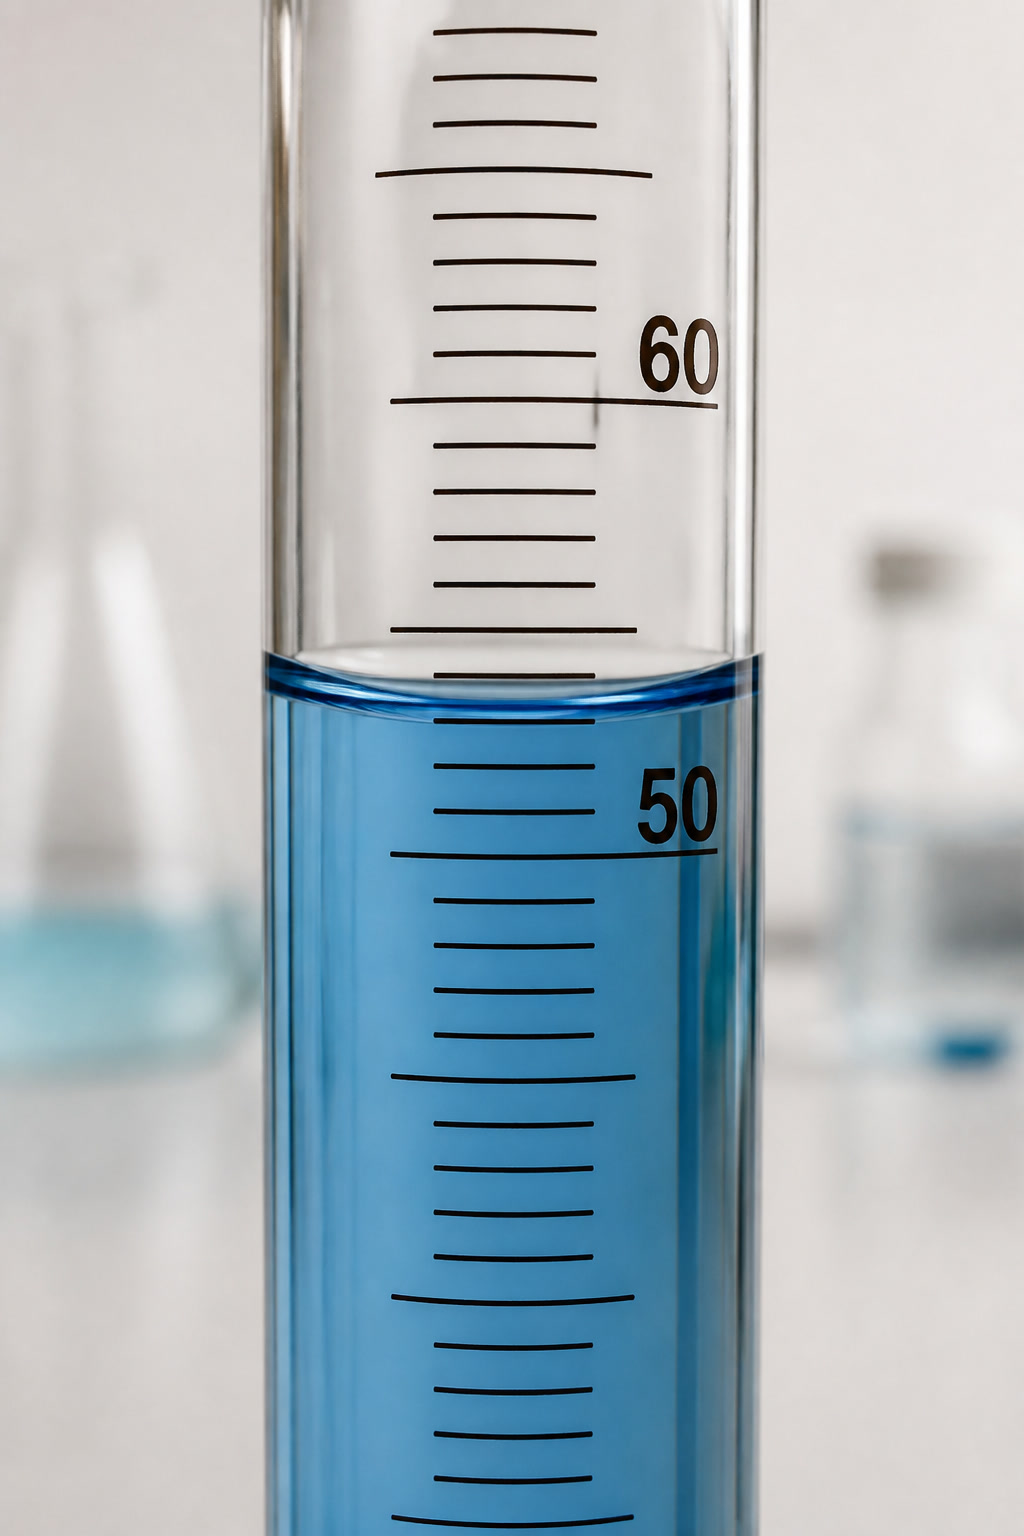
\includegraphics[width=0.3\linewidth]{images/book1/ai/g6-volume-cylinder.jpg}

{\small De \omterm{met:g6:mass-and-volume:cylinder}{meniscus} van dichtbij: lees het vlakke midden van de kromming af, met je oog op die hoogte.}
\end{omfigure}

\section{Vaste stoffen meten --- zelfs bobbelige}

Een baksteenvormige \omterm{def:g3:solids-liquids-gases:solid}{vaste stof} geeft zich over aan de liniaal: lengte
maal breedte maal hoogte geeft haar \omterm{def:g6:mass-and-volume:volume}{volume} in \unit{cm^3}, zoals je
wiskundecursus liet zien. Maar wat met een kiezelsteen, een sleutel,
een pruim? Geen liniaal past om een bobbel. Het antwoord is
tweeduizend jaar oud, en het kwam uit een badkuip.

\begin{proposition}[Verdringing]\label{prop:g6:mass-and-volume:displacement}
Een \omterm{def:g3:solids-liquids-gases:solid}{vaste stof} die helemaal onder water wordt gebracht, duwt precies
zijn eigen \omterm{def:g6:mass-and-volume:volume}{volume} aan water opzij --- hij verdringt het. De stijging
van het waterniveau meet de indringer: bobbelig of glad, het water
vormt zich naar elke deuk en elke bult.
\end{proposition}

\begin{method}[Volume uit de stijging van het water]\label{met:g6:mass-and-volume:rise}
\begin{enumerate}
  \item giet water in een maatcilinder --- genoeg om het voorwerp te
        bedekken --- en lees het \omterm{def:g6:mass-and-volume:volume}{volume} af: zeg \qty{120}{mL};
  \item bind een draadje aan het voorwerp en laat het voorzichtig
        zakken tot het helemaal onder water is, zonder plons en
        zonder de wanden te raken;
  \item lees opnieuw af: zeg \qty{145}{mL};
  \item trek af: $145 - 120 = 25$ --- het \omterm{def:g6:mass-and-volume:volume}{volume} van het voorwerp is
        \qty{25}{cm^3} (milliliters stijging, centimeterkubusjes
        steen: hetzelfde ding).
\end{enumerate}
\end{method}

\begin{omfigure}
\begin{tikzpicture}[scale=0.85]
  \draw[thick] (0.8,0) -- (0.8,3.6) (2.6,0) -- (2.6,3.6)
    (0.8,0) -- (2.6,0);
  \fill[omDef, opacity=0.2] (0.8,0.05) rectangle (2.6,2.0);
  \draw[omDef, very thick] (0.8,2.0) -- (2.6,2.0);
  \node[right, font=\footnotesize] at (2.7,2.0) {120};
  \node[below, font=\small] at (1.7,-0.3) {ervoor};
  \draw[thick] (6.2,0) -- (6.2,3.6) (8.0,0) -- (8.0,3.6)
    (6.2,0) -- (8.0,0);
  \fill[omDef, opacity=0.2] (6.2,0.05) rectangle (8.0,2.42);
  \draw[omDef, very thick] (6.2,2.42) -- (8.0,2.42);
  \node[right, font=\footnotesize] at (8.1,2.42) {145};
  \draw (7.1,3.6) -- (7.1,1.0);
  \fill[omExo] (7.1,0.75) ellipse (0.4 and 0.3);
  \node[below, font=\small] at (7.1,-0.3)
    {erna: de kiezel, helemaal onder};
  \draw[-Stealth, omThm, thick] (4.0,2.0) -- (5.6,2.35);
  \node[below, font=\small, omThm] at (4.8,1.9)
    {stijging: \qty{25}{mL}};
\end{tikzpicture}

{\small De stijgmethode: het water klimt precies met het \omterm{def:g6:mass-and-volume:volume}{volume} van
de kiezel --- $145 - 120 = \qty{25}{cm^3}$ kiezel.}
\end{omfigure}

\begin{example}[De kroon in de badkuip]\label{ex:g6:mass-and-volume:archimedes}
Het oude verhaal: een koning vermoedde dat zijn goudsmid het goud van
de koninklijke kroon met zilver had verdund, en vroeg de geleerde
Archimedes dat uit te zoeken zonder de kroon te beschadigen. Toen hij
in een vol bad stapte, zag Archimedes het water over de rand klotsen
--- en zag hij in een flits dat de overloop het \omterm{def:g6:mass-and-volume:volume}{volume} van zijn eigen
lichaam mat, bobbels en al. De legende zegt dat hij door de straten
rende en ``Eureka!'' riep --- \emph{ik heb het gevonden!} Hoe het
\omterm{def:g6:mass-and-volume:volume}{volume} van de kroon het bedrog ontmaskerde heeft nog één idee nodig,
twee hoofdstukken verderop; de badkuip gaf hem het \omterm{def:g6:mass-and-volume:volume}{volume} van
\emph{alles}.
\end{example}

\section{Massa en volume zijn verschillende antwoorden}

\begin{example}[Zelfde volume, andere massa]\label{ex:g6:mass-and-volume:different}
Vul twee identieke glazen van \qty{25}{cL}, het ene met water, het
andere met honing, en weeg ze (de glazen eraf getrokken): het
honingglas bevat merkbaar meer \omterm{def:g3:measuring-mass:units}{gram} in precies dezelfde ruimte. Zelfde
\omterm{def:g6:mass-and-volume:volume}{volume}, andere \omterm{def:g3:measuring-mass:mass}{massa}. En een \omterm{def:g6:mass-and-volume:volume}{liter} \omterm{def:g2:air-around-us:air}{lucht} weegt nauwelijks meer
dan een \omterm{def:g3:measuring-mass:units}{gram}, in de ruimte waar een \omterm{def:g6:mass-and-volume:volume}{liter} water een hele
\omterm{def:g3:measuring-mass:units}{kilogram} weegt. Ruimte en stof zijn werkelijk verschillende
boekhouders --- houd die gedachte stevig vast: ze wordt een wet, met
een naam, in het laatste hoofdstuk van dit jaar.
\end{example}

\begin{remark}[Wegen wat niet alleen kan staan]\label{rem:g6:mass-and-volume:tare}
Hoe weeg je bloem zonder haar kom mee te wegen? Moderne balansen
hebben er een knop voor: zet de lege kom op de schaal, druk --- de
display springt terug naar nul --- en schep dan: de balans meldt nu de
bloem alleen. Die handeling heet \emph{tarreren}. Zonder knop weeg je
twee keer en trek je af: kom-met-bloem min lege kom. Hoe dan ook is
het opnieuw de eerlijke-startregel: begin vanaf een eerlijke nul.
\end{remark}

\section{Oefeningen}

\begin{exercise}[$\star$]\label{exo:g6:mass-and-volume:1}
Welke vraag beantwoordt \omterm{def:g6:mass-and-volume:volume}{volume}, en welke vraag beantwoordt
\omterm{def:g3:measuring-mass:mass}{massa}? Geef van elk de twee voornaamste eenheden.
\end{exercise}

\begin{exercise}[$\star$]\label{exo:g6:mass-and-volume:2}
Reken om: \qty{2}{L} naar \unit{cm^3}; \ \qty{350}{mL} naar
\unit{cm^3}; \ \qty{1500}{cm^3} naar \omterm{def:g6:mass-and-volume:volume}{liter}; \ een halve
\omterm{def:g6:mass-and-volume:volume}{liter} naar milliliter.
\end{exercise}

\begin{exercise}[$\star$]\label{exo:g6:mass-and-volume:3}
Waarom moet je een maatcilinder op ooghoogte, op de tafel en bij de
onderkant van de \omterm{met:g6:mass-and-volume:cylinder}{meniscus} aflezen? Noem de fout die elke regel
voorkomt.
\end{exercise}

\begin{exercise}[$\star$]\label{exo:g6:mass-and-volume:4}
Een cilinder wijst \qty{200}{mL} aan; met een pruim erin gelaten wijst
hij \qty{265}{mL} aan. Wat is het \omterm{def:g6:mass-and-volume:volume}{volume} van de pruim, in
\unit{cm^3}?
\end{exercise}

\begin{exercise}[$\star$]\label{exo:g6:mass-and-volume:5}
Waarom werkt de stijgmethode zelfs voor een bobbelige kiezelsteen,
terwijl geen liniaal hem kon \omterm{def:g6:measurement-in-science:measuring}{meten}? Welke propositie geeft het
antwoord?
\end{exercise}

\begin{exercise}[$\star$]\label{exo:g6:mass-and-volume:6}
Een baksteenvormige gum meet \qty{5}{cm} bij \qty{2}{cm} bij
\qty{1}{cm}. Zijn \omterm{def:g6:mass-and-volume:volume}{volume}? Controleplan: hoe zou je het met de
stijgmethode bevestigen?
\end{exercise}

\begin{exercise}[$\star$]\label{exo:g6:mass-and-volume:7}
Rijst wegen: lege kom \qty{280}{g}; kom met rijst \qty{745}{g}.
Hoeveel rijst? Welke knop doet hetzelfde werk in één stap?
\end{exercise}

\begin{exercise}[$\star$]\label{exo:g6:mass-and-volume:8}
Wat heeft het grootste \omterm{def:g6:mass-and-volume:volume}{volume}, een \omterm{def:g3:measuring-mass:units}{kilogram} veren of een
\omterm{def:g3:measuring-mass:units}{kilogram} ijzer? Wat heeft de grootste \omterm{def:g3:measuring-mass:mass}{massa}? (Beantwoord beide
zorgvuldig.)
\end{exercise}

\begin{exercise}[$\star\star$]\label{exo:g6:mass-and-volume:9}
De stijgmethode faalt bij een kurk: die \omterm{def:g1:floating-and-sinking:words}{drijft}. Stel een oplossing
voor die de cilinder toch gebruikt --- en zeg wat er moet worden
afgetrokken als je oplossing een hulpvoorwerp gebruikt.
\end{exercise}

\begin{exercise}[$\star\star$]\label{exo:g6:mass-and-volume:10}
Op een pak sap staat \qty{1}{L}. Uitgeschonken vult het drie keer een
glas van \qty{250}{mL}, en het vierde glas maar tot het streepje
\qty{200}{mL}. Was de bewering eerlijk? Hoeveel scheelde het?
\end{exercise}

\begin{exercise}[$\star\star$]\label{exo:g6:mass-and-volume:11}
Een halsketting wordt in een cilinder gelaten die \qty{80.0}{mL}
aanwijst; hij stijgt tot \qty{83.5}{mL}. De juwelier beweert dat de
ketting \qty{5}{cm^3} goud bevat. Kan die bewering waar zijn? Wat
heeft het water precies gemeten?
\end{exercise}

\begin{exercise}[$\star\star\star$]\label{exo:g6:mass-and-volume:12}
Ontwerp een badkuipachtige controle van
\cref{prop:g6:mass-and-volume:displacement} zelf, met een
baksteenvormig voorwerp waarvan de liniaal het \omterm{def:g6:mass-and-volume:volume}{volume} al kent.
Beschrijf de stappen, voorspel de twee aflezingen van de cilinder voor
een blokje van $4 \times 3 \times 2$ \omterm{def:g2:measuring-length:units}{centimeter} dat in
\qty{150}{mL} wordt gelaten, en zeg welk resultaat de propositie
onderuit zou halen.
\end{exercise}

\section{Probleem: bottelen op de boomgaard}

\begin{problem}[{Weekendprobleem --- persdag op de boomgaard; liters in
flessen, kratten op de weegschaal; de kiezel in de
kan}]\label{pb:g6:mass-and-volume:1}
De boomgaard perst vandaag zijn appels, en elke helper krijgt een
meetklus.

\medskip\noindent\textbf{Deel I --- Sap per \omterm{def:g6:mass-and-volume:volume}{liter}.}
De pers heeft een vat van \qty{20}{L} gevuld.
\begin{enumerate}
  \item Hoeveel \omterm{def:g6:mass-and-volume:volume}{kubieke centimeter} is \qty{20}{L}?
  \item Het sap wordt gebotteld in flessen van \qty{75}{cL}. Hoeveel
        \emph{volle} flessen levert het vat op?
  \item Hoeveel sap blijft er na de laatste volle fles over, in
        centiliter?
  \item Het restje wordt in glazen van \qty{25}{cL} geschonken.
        Hoeveel glazen vult het?
\end{enumerate}

\medskip\noindent\textbf{Deel II --- Kratten op de weegschaal.}
\begin{enumerate}[resume]
  \item Een lege fles heeft \omterm{def:g3:measuring-mass:mass}{massa} \qty{450}{g}. Wat is met Deel I de
        \omterm{def:g3:measuring-mass:mass}{massa} van het sap in één volle fles, als een \omterm{def:g6:mass-and-volume:volume}{liter} sap een
        \omterm{def:g3:measuring-mass:mass}{massa} van ongeveer \qty{1}{kg} heeft? (Reken in \omterm{def:g3:measuring-mass:units}{gram}.)
  \item Wat weegt één volle fles dus in totaal?
  \item Een houten krat weegt leeg \qty{2}{kg} en draagt zes volle
        flessen. Totale \omterm{def:g3:measuring-mass:mass}{massa} van een geladen krat?
  \item Het busje mag \qty{200}{kg} aan kratten vervoeren. Hoeveel
        geladen kratten mag het meenemen? (Alleen hele kratten.)
\end{enumerate}

\medskip\noindent\textbf{Deel III --- De kiezel in de kan.}
Kleine Tom laat een kiezelsteen in een volle kan sap van \qty{1}{L}
vallen, en er stroomt sap over de tafel.

\begin{enumerate}[resume]
  \item Het opgedweilde overgelopen sap meet \qty{40}{mL}. Wat heeft
        de gemorste hoeveelheid over de kiezel gemeten, en volgens
        welke propositie?
  \item Hoeveel sap blijft er in de kan nadat de kiezel eruit is
        gevist?
  \item Tom protesteert: ``De kiezel is klein --- kijk, hij past in
        mijn vuist!'' Zijn zus antwoordt met een maatcilinder: ze
        legt de kiezel in \qty{100}{mL} water. Welke aflezing bewijst
        dat het gemorste sap de waarheid vertelde?
  \item Bonusboekhouding: de kiezel weegt \qty{104}{g} op de
        keukenweegschaal. Kun je zonder enig nieuw idee al zeggen of
        kiezelstof zwaarder of lichter is dan sapstof \emph{voor
        dezelfde ingenomen ruimte}? Vergelijk \qty{104}{g} kiezel in
        \qty{40}{cm^3} met de \omterm{def:g3:measuring-mass:mass}{massa} sap die diezelfde
        \qty{40}{cm^3} zou vullen --- en houd je conclusie warm voor
        het hoofdstuk over dichtheid.
\end{enumerate}
\end{problem}
